% !Mode:: "TeX:UTF-8"
% !TEX program  = xelatex
% !BIB program  = biber
\documentclass[AutoFakeBold,AutoFakeSlant,language=chinese,degree=bachelor]{sustechthesis}
% 1. AutoFakeBold 与 AutoFakeSlant 为伪粗与伪斜,如果本机上有相应粗体与斜体字体,请使用 xeCJK 宏包进行设置,例如:
%   \setCJKmainfont[
%     UprightFont = * Light,
%     BoldFont = * Bold,
%     ItalicFont = Kaiti SC,
%     BoldItalicFont = Kaiti SC Bold,
%   ]{Songti SC}
%
% 2. language=chinese 基于为 ctexart 文类提供的中文排版方案修改,如果使用英文进行论文创作,请使用 language=english 选项。
%
% 3. degree=bachelor 为 sustechthesis 文类提供的本科生毕业论文模板,其他可选项为 master 与 doctor,但是均未实现,如果您对此有兴趣,欢迎 PR。
%
% 4. sustechthesis.cls 文类主要参考自去年完成使命的 sustechthesis.tex,在这一年的时间,作者的 TeX 风格与常用宏包发生许多变化,因为之前的思想为仅提供必要的格式修改相关代码,所以转换为文类形式所进行的修改较少,而近期的风格与常用宏包均体现在以下的例子文件中。
%
% 5. 示例文件均放置于相应目录的 examples 文件夹下,构建自己论文时可暂时保留,用以检索接口与使用方法。
%
% 6. 英文目录需要居中可以使用:\renewcommand{\contentsname}{\centerline{Content}}
%
% 7. LaTeX 中公式编号括号样式及章节关联的方法:https://liam.page/2013/08/23/LaTeX-Formula-Number/

% !Mode:: "TeX:UTF-8"
% !TEX program  = xelatex

% 数学符号与环境
\usepackage{amsmath,amssymb}
  \newcommand{\dd}{\mathrm{d}}
  \newcommand{\RR}{\mathbb{R}}
% 参考文献
\usepackage[style=gb7714-2015,gbpunctin=false]{biblatex}
  \addbibresource{ref.bib}
% 公式按照章节标号
\usepackage{amsmath}
\numberwithin{equation}{section}
% caption居中
\usepackage[justification=centering]{caption}
% 页眉
\usepackage{fancyhdr}

\fancypagestyle{mystyle}{
    \fancyhf{}
    \fancyhead[C]{\宋体\小五 论文标题(修改config/preamble.tex 21行)} % 页眉添加文章题目
    \renewcommand{\headrulewidth}{0.2pt} % 分隔线宽度0.2磅
    \fancyfoot[C]{\thepage} % 在页脚中间添加页码
}

% \fancyhead[C]{\宋体\小五 点接触式双足机器人的动态行走算法研究}
% \renewcommand{\headrulewidth}{0.4pt}%分隔线宽度4磅
% 无意义文本
\usepackage{zhlipsum,lipsum}
% 列表环境设置
\usepackage{enumitem}
% 浮动题不越过 \section
\usepackage[section]{placeins}
% 超链接
\usepackage{hyperref}
% 图片,子图,浮动题设置
\usepackage{graphicx,subcaption,float}
% 抄录环境设置,更多有趣例子请命令行输入 `texdoc tcolorbox`
\usepackage{tcolorbox}
  \tcbuselibrary{xparse}
  \DeclareTotalTCBox{\verbbox}{ O{green} v !O{} }%
    {fontupper=\ttfamily,nobeforeafter,tcbox raise base,%
    arc=0pt,outer arc=0pt,top=0pt,bottom=0pt,left=0mm,%
    right=0mm,leftrule=0pt,rightrule=0pt,toprule=0.3mm,%
    bottomrule=0.3mm,boxsep=0.5mm,bottomrule=0.3mm,boxsep=0.5mm,%
    colback=#1!10!white,colframe=#1!50!black,#3}{#2}%
\tcbuselibrary{listings,breakable}
  \newtcbinputlisting{\Python}[2]{
    listing options={language=Python,numbers=left,numberstyle=\tiny,
      breaklines,commentstyle=\color{white!50!black}\textit},
    title=\texttt{#1},listing only,breakable,
    left=6mm,right=6mm,top=2mm,bottom=2mm,listing file={#2}}
% 三线表支持
\usepackage{booktabs}

% LaTeX logo
\usepackage{hologo}
 % 导言区
% !Mode:: "TeX:UTF-8"
% !TEX program  = xelatex
\设置信息{
    % 键 = {{中文值}, {英文值}},
    % 分类号 = {{}, {}},
    % 编号 = {{}, {}},
    % UDC = {{}, {}},
    % 密级 = {{}, {}},
    % 仅题目(不含副标题)、系别、专业,支持手动 \\ 换行,不支持自动换行。
    题目 = {{南方科技大学本科生毕业论文模板\\2024年机械系非官方版本}, {Graduation Thesis Template \\2024 MEE Unofficial Version}},
    % 如无需副标题,删除值内容即可,不可删除键定义。
    % 副标题 = {{}, {}},
    姓名 = {{付成龙}, {Chenglong Fu}},
    学号 = {{12010000}, {12010000}},
    系别 = {{机械与能源工程}, {Department of Mechanical \\and Energy Engineering}},
    专业 = {{机器人工程}, {Robotics Engineering}},
    指导老师 = {{融亦鸣}, {Yiming Rong}},
    时间 = {{2024年5月x日}, {May x, 2024}},
    职称 = {{教授}, {Professor}},
}
 % 论文信息

\begin{document}

\中文标题页
\英文标题页

\中文诚信承诺书
\英文诚信承诺书

\前序格式化

\摘要标题
% !Mode:: "TeX:UTF-8"
% !TEX program  = xelatex
\begin{中文摘要}{\LaTeX ;接口}
  此本科生\LaTeX 毕业论论模板,按照2024年机械系给出的本科生毕业设计论文word模板修改,基于sustechthesis项目\footnote{https://github.com/iydon/sustechthesis}。这个模板最初由笔者在撰写毕业论文时创建,由于2024年机械系给出的word模板和sustechthesis项目中有一些差异,而笔者的毕业设计是在ubuntu平台上开发的,若使用word则不方便论文写作。于是在笔者毕业设计论文写作完成之后,整理了此模板,以供之后的同学参考。因为使用了此模板而导致的任何问题和后果,笔者概不负责。最后,由于笔者\LaTeX 水平有限,未来有时间的话会继续维护该模板,同时欢迎对此模板进行意见反馈,希望各位不吝赐教。
\end{中文摘要}

\begin{英文摘要}{LaTeX, Interface}
  \lipsum[1]
\end{英文摘要}
 % 论文摘要

\目录\clearpage % 目录及换页

\正文格式化
% !Mode:: "TeX:UTF-8"
% !TEX program  = xelatex
\section{免责声明}
\begin{enumerate}[label={\alph*)}]
    \item 本模板的发布遵守 \LaTeX\ Project Public License,使用前请认真阅读协议内容。
    \item 南方科技大学教学工作部只提供毕业论文写作指南,不提供官方模板,也不会授权第三方模板为官方模板,所以此模板仅为写作指南的参考实现,不保证格式审查老师不提意见. 任何由于使用本模板而引起的论文格式审查问题均与本模板作者无关。
    \item 任何个人或组织以本模板为基础进行修改,扩展而生成的新的专用模板,请严格遵守 \LaTeX\ Project Public License 协议。由于违犯协议而引起的任何纠纷争端均与本模板作者无关。
\end{enumerate}
\clearpage
% !Mode:: "TeX:UTF-8"
% !TEX program  = xelatex
\section{文类接口}
文类的接口的命名均为汉字,意思为字面意思,如有疑问,欢迎在 GitHub 提出 \href{https://github.com/Iydon/sustechthesis/issues}{Issues}。

\subsection{汉化字号接口}
本接口主要使用 \texttt{ctex} 宏包。

\verbbox{\初号},\verbbox{\小初},\verbbox{\一号},\verbbox{\小一},\verbbox{\二号},\verbbox{\小二},\verbbox{\三号},\verbbox{\小三},\verbbox{\四号},\verbbox{\小四},\verbbox{\五号},\verbbox{\小五},\verbbox{\六号},\verbbox{\小六},\verbbox{\七号},\verbbox{\八号}。


\subsection{汉化字体接口}
可能本机上部分字体不存在,导致部分字体无法使用。

\verbbox{\宋体},\verbbox{\黑体},\verbbox{\仿宋},\verbbox{\楷书},\verbbox{\隶书},\verbbox{\幼圆},\verbbox{\雅黑},\verbbox{\苹方}。


\subsection{字体效果接口}

建议在正文时使用 \verb|\textbf{}|,\verb|\textit{}| 调用\textbf{粗体}与\textit{斜体}。

It is recommended to use \verb|\textbf{}|,\verb|\textit{}| to call \textbf{Bold} and \textit{ItalicFont}.

\verbbox{\粗体},\verbbox{\斜体}。


\subsection{格式相关接口}
\subsubsection{命令}
例子请参考前文,在写论文初期,可以注释掉标题页等不必要信息,以加快编译速度。

\verbbox{\设置信息},\verbbox{\目录},\verbbox{\下划线},\verbbox{\中文标题页},\verbbox{\英文标题页},\verbbox{\中文诚信承诺书},\verbbox{\英文诚信承诺书},\verbbox{\摘要标题},\verbbox{\参考文献},\verbbox{\附录},\verbbox{\致谢}。

\subsubsection{环境}
摘要环境均需一个参数,为关键词:\verb|\begin{}...\end{}|。

\verbbox{中文摘要},\verbbox{英文摘要}。
\clearpage
% !Mode:: "TeX:UTF-8"
% !TEX program  = xelatex

\section{一些样例}

以下,笔者结合自己的使用习惯和经验添加了一些内容。
\subsection{图片}

如图\ref{fig.test_figure},是一张测试图片。
\begin{figure}[htb]
    \centering
    \includegraphics[width=.5\textwidth]{example-image-a}
    \caption{自带测试图片---Test image}\label{fig.test_figure}
    % 图片的标题应该在下方
\end{figure}

如图\ref{fig.shu_and_kun},是一只鼠鼠和一值坤坤。如图\ref{fig.shushu},是一只鼠鼠。如图\ref{fig.kunkun},是一只坤坤。

\begin{figure}[htb]
    \centering
    \begin{subfigure}[t]{.35\textwidth}
        \centering
        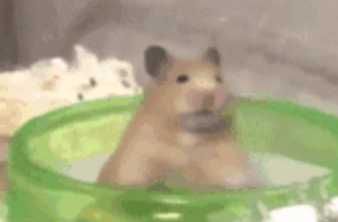
\includegraphics[width=1\textwidth]{figures/shushu.png}
        \caption{这是一只鼠鼠}\label{fig.shushu}
    \end{subfigure}
    \begin{subfigure}[t]{.35\textwidth}
        \centering
        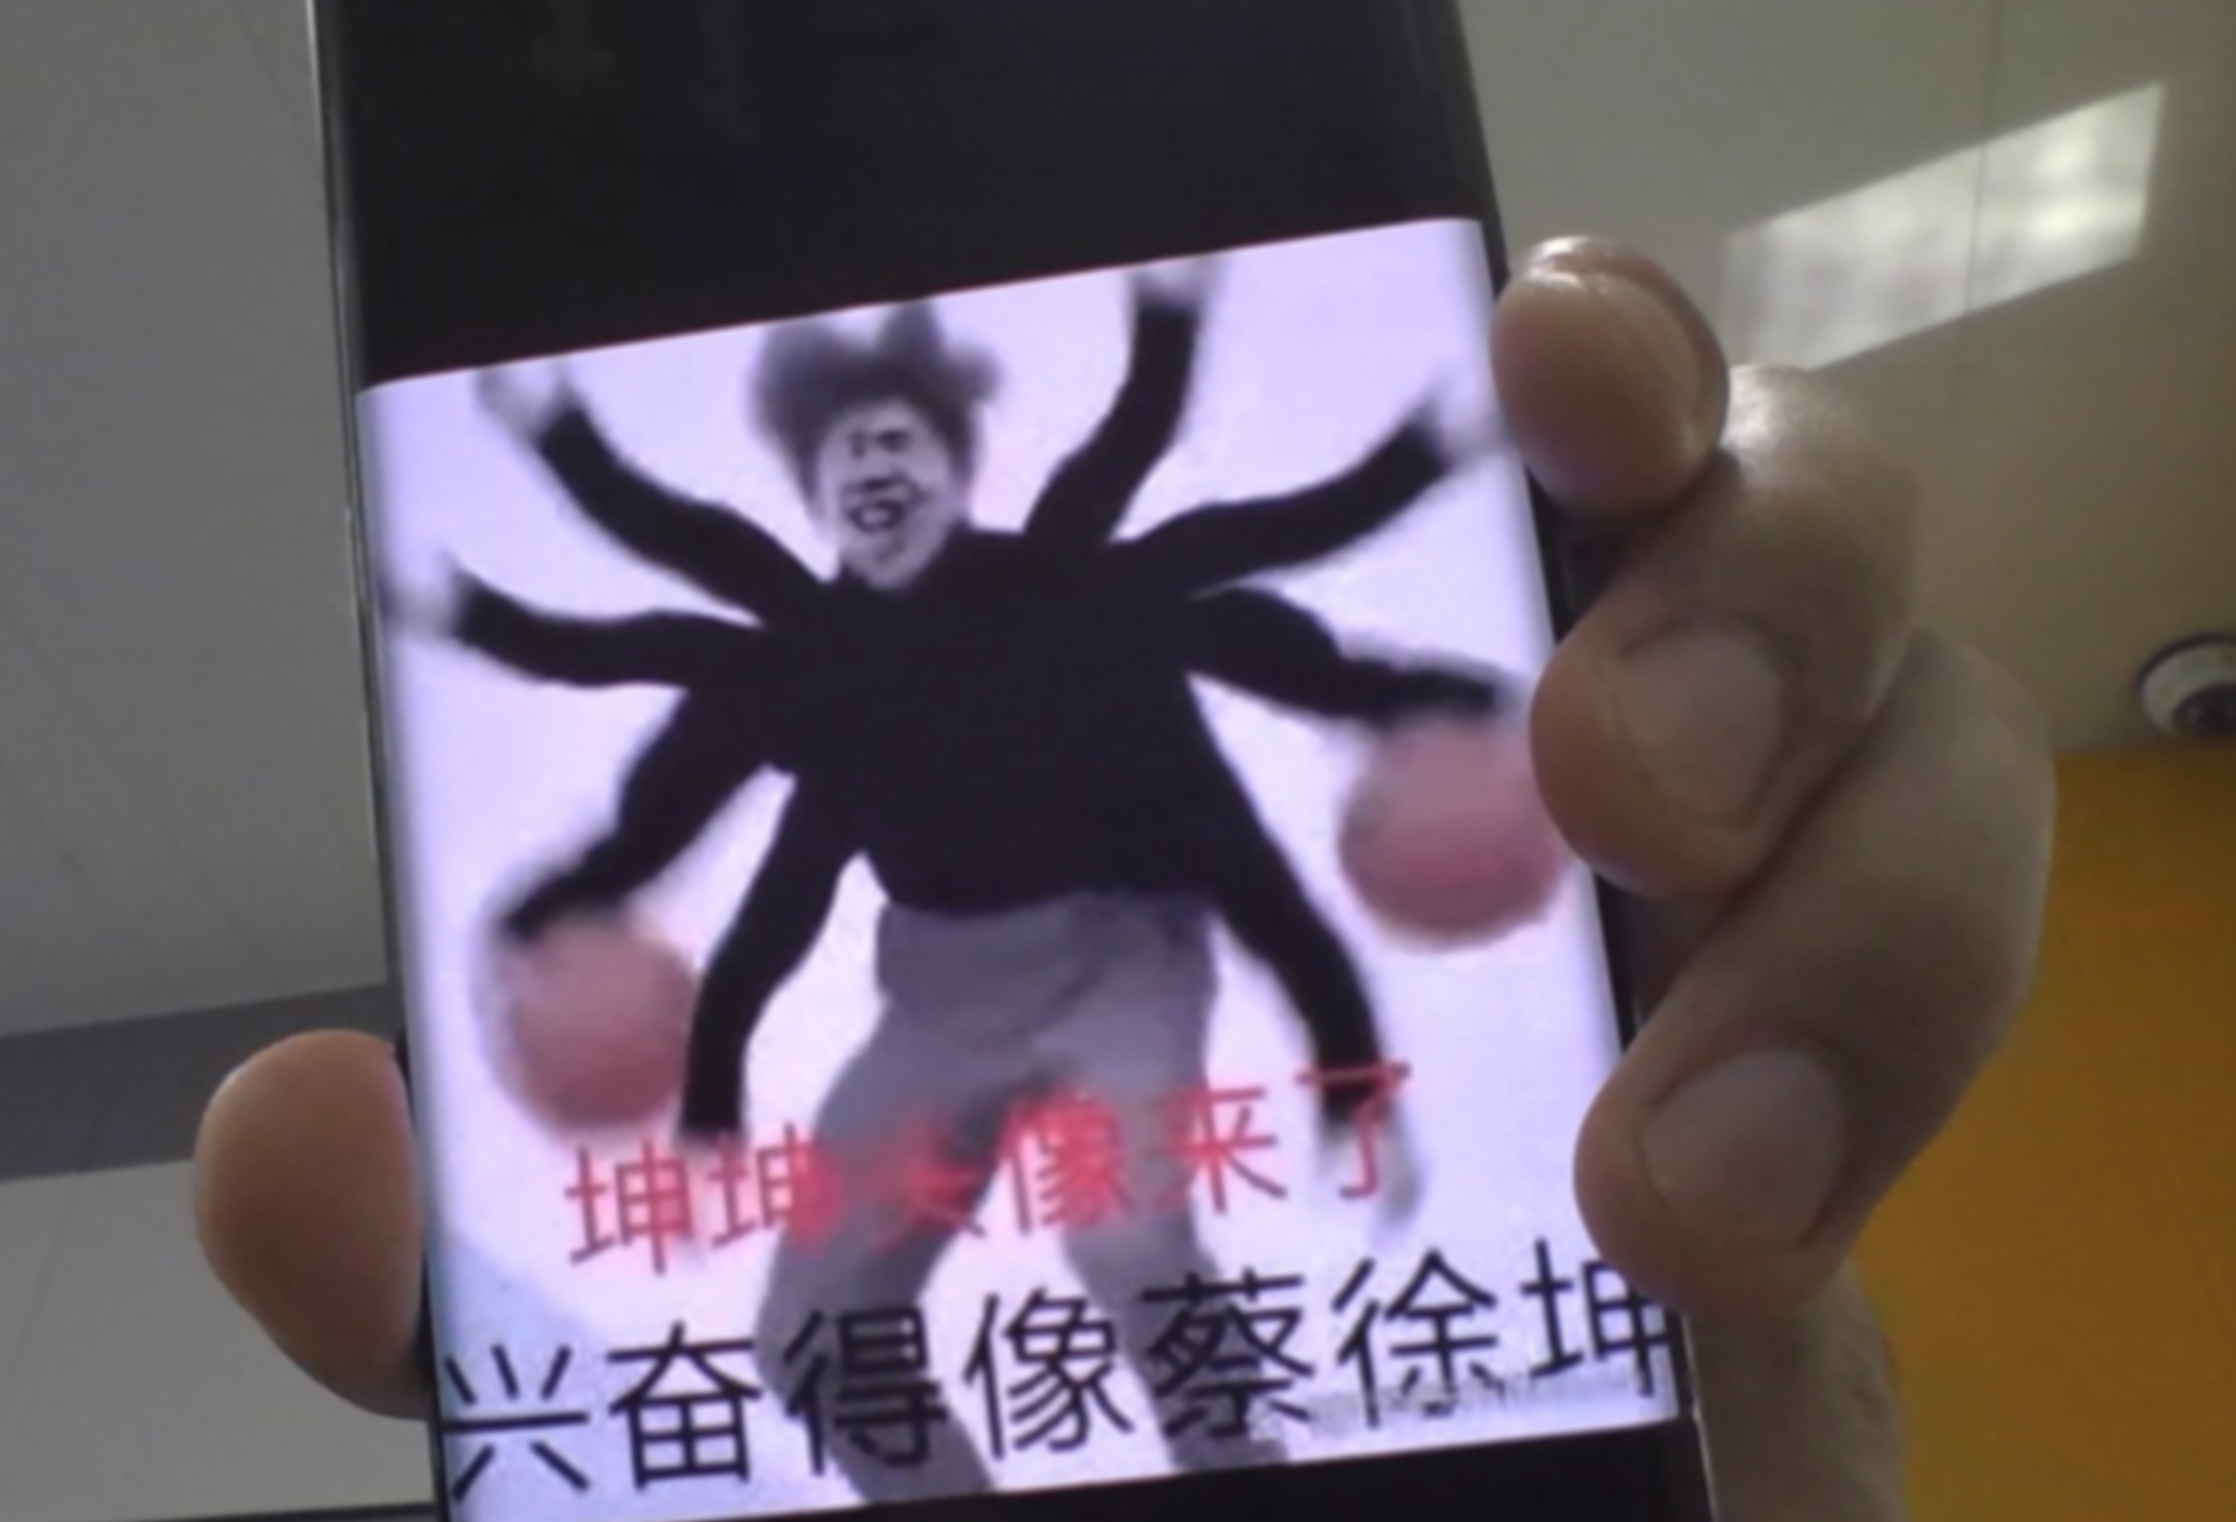
\includegraphics[width=1\textwidth]{figures/kunkun.png}
        \caption{这是一只坤坤,他在说只因你太美,baby}\label{fig.kunkun}
    \end{subfigure}

    \caption{鼠鼠和坤坤}\label{fig.shu_and_kun}
\end{figure}

\subsection{公式}

公式推荐使用\verb|\begin{equation}...\end{equation}|  和\verb|\begin{align}...\end{align}|包裹。在align环境中,不需要标明的公式号的行在末尾处要添加\verb|\nonumber|


示例如下:

\begin{equation}
    \mathbf{M}\begin{pmatrix}\ddot{\mathbf{q}}_f\\\ddot{\mathbf{q}}_j\end{pmatrix}+\mathbf{h}(\mathbf q,\mathbf {\dot q})+\mathbf{g}=\begin{pmatrix}\mathbf{0}_6\\\boldsymbol{\tau}\end{pmatrix}+\boldsymbol{J}_c^\top\mathbf{f}_r
\end{equation}

\begin{align}
    J   & =  ||\Delta \mathbf f||^2_{\mathbf{Q_1}} + ||\Delta \mathbf b||^2_{\mathbf{Q_1}} 
                                \nonumber \\ 
        & =  \begin{bmatrix}
            \Delta \mathbf f \\
            \Delta \mathbf b \\
        \end{bmatrix}^\intercal 
        \begin{bmatrix}
            \mathbf{Q_1} & \\
            & \mathbf{Q_2} \\
        \end{bmatrix}
        \begin{bmatrix}
            \Delta \mathbf f \\
            \Delta \mathbf b \\
        \end{bmatrix} 
                               \nonumber  \\
        & =  \mathbf{u}^\intercal \mathbf H \mathbf{u} + 2\mathbf{u}^\intercal\mathbf h
\end{align}


\subsection{表格}

表格与图片可以直接通过\verbbox{\ref{<key>}}来引用,例如表\ref{table2}、图\ref{F:test-a}、图\ref{F:test-b-sub-b}。

\begin{table}[htb]
% h-here,t-top,b-bottom,优先级依次下降
    % 居中,模版已设定表格浮动体居中
    \centering
    \caption{表格的标题应该放在上方}
    \label{table}
    \begin{tabular}{lc} % 三线表不能有竖线,l-left,c-center,r-right
        \toprule
        %三线表-top 线
        Example & Result \\
        \midrule
        %三线表-middle 线
        Example1          & 0.25 \\
        Example2          & 0.36 \\
        \bottomrule
        %三线表-底线
    \end{tabular}
\end{table}

\begin{table}[htb]
    \centering
    \caption{带表注的表格的标题}
    \label{table2}
    \begin{threeparttable}
        \setlength{\tabcolsep}{0.6cm}{ % 调节表格长度
                \begin{tabular}{lc} % 三线表不能有竖线,l-left,c-center,r-right
                    \toprule
                    %三线表-top 线
                    Example & Result \\
                    \midrule
                    %三线表-middle 线
                    Example1          & 0.25\tnote{1} \\
                    Example2          & 0.36 \\
                    \bottomrule
                    %三线表-底线
                \end{tabular}
        }
        \begin{tablenotes}
            \item[1] 数据来源:南方科技大学 \LaTeX 模版 % 增加表格数据来源注释
        \end{tablenotes}
    \end{threeparttable}
\end{table}

\subsection{参考文献}

参考文献一般使用\verbbox{\cite{<key>}}命令,效果如是\cite{Nicholas1998Handbook},sustechthesis\cite{sustechthesis}。引用作者使用\verbbox{\citeauthor{<key>}},效果如是“\citeauthor{goossens1994latex}”。
\clearpage
% !Mode:: "TeX:UTF-8"
% !TEX program  = xelatex
\section{\LaTeX\ 入门}
请参考 \href{https://tex.readthedocs.io/zh_CN/latest/}{在线文档},包括学习资源及学习路径。欢迎在 GitHub 上提出 \href{https://github.com/Iydon/tex/issues}{Issues}。
\clearpage

\参考文献
  \printbibliography[heading=none]\clearpage
\附录
  % !Mode:: "TeX:UTF-8"
% !TEX program  = xelatex
\section*{数据获取函数}\label{A:data}
\Python{utils.py}{code/examples/utils.py}
\clearpage
\致谢
  % !Mode:: "TeX:UTF-8"
% !TEX program  = xelatex
感谢\sustechthesis\ 项目为南方科技大学校友提供的便利。以下是\sustechthesis\ 项目参与人员。
\begin{itemize}
    \item 梁钰栋(南方科技大学,本科 17 级);
    \item 张志炅(南方科技大学,本科 17 级)。
\end{itemize}
以及使用本项目,并提出诸多宝贵的修改意见的使用人员们:
\begin{itemize}
    \item 李未晏(南方科技大学,本科 15 级);
    \item 张尔聪(南方科技大学,本科 15 级)。
\end{itemize}

笔者并非计算机系,可能存在对协议等的错误使用,如果你在本模板中发现任何问题,请在 GitHub 中提交Issue,同时也非常欢迎对该模板的贡献!

\end{document}
